\documentclass[a4paper, 15pt, oneside]{article}
\linespread{1.15} %interlinea
\pagestyle{plain}
\usepackage{geometry} %margini
\usepackage[]{tabto}
\geometry{a4paper, top=3cm, bottom=3cm, left=3cm, right=3cm, bindingoffset=5mm}
\usepackage{graphicx}
\graphicspath{Documentazione/Immagini/}
\usepackage{multicol} %più colonne
\usepackage{ragged2e} %allineamento testo
\usepackage{float}
\author{Gioele Manzoni}
\title{Documentazione per Progettazione Base di Dati}
\begin{document}
	\begin{center}
		\begin{figure}[hb]
			
\includegraphics[width=1\textwidth]{Immagini/coverpic}
		\end{figure}
		{\LARGE DOCUMENTAZIONE PER PROGETTAZIONE \\ OBJECT ORIENTATION \par}
		{\Large{Progetto in Carico: Hackathon \par}}
		\vfill
		{\large{ \textbf{\textsc{CdL Triennale in Informatica}}}}\\
		{\large{\textsc{Corso di Object Orientation}}}\\
		{\large{\textsc{GIOELE MANZONI}}}\\
		{\large{\textsc{N86004562}}}\\
		{\large{\textsc{LUCA LUCCI}}}\\
		{\large{\textsc{N86005180}}}\\
		{\large{\textsc{\today}}}\\
		\Large{\textsc{Anno Accademico: 2024/2025}}
	\end{center}
	\newpage
	\tableofcontents
	\newpage
	\section{Traccia Progetto: Hackathon}
	Un Hackathon, ovvero una "maratona di hacking", è un evento durante il quale team di partecipanti si sfidano per progettare e implementare nuove soluzioni basate su una certa tecnologia o mirate a un certo ambito applicativo. 
	Ogni Hackathon ha un titolo identificativo, si svolge in una certa sede e in un certo intervallo di tempo (solitamente 2 giorni) e ha un organizzatore specifico (registrato alla piattaforma). L'organizzatore seleziona un gruppo di giudici (selezionati tra gli utenti della piattaforma, invitandoli). Infine, l'organizzatore apre le registrazioni, che si chiuderanno 2 giorni prima dell'evento. Ogni evento avrà un numero massimo di iscritti e una dimensione massima del team.
	Durante il periodo di registrazione, gli utenti possono registrarsi per l'Hackathon di loro scelta (eventualmente registrandosi sulla piattaforma se non lo hanno già fatto). Una volta iscritti, gli utenti possono formare team. I team diventano definitivi quando si chiudono le iscrizioni. All'inizio dell'hackathon, i giudici pubblicano una descrizione del problema da affrontare. 
	Durante l'hackathon, i team lavorano separatamente per risolvere il problema e devono caricare periodicamente gli aggiornamenti sui "progressi" sulla piattaforma come documento, che può essere esaminato e commentato dai giudici. Alla fine dell'hackathon, ogni giudice assegna un voto (da 0 a 10) a ciascun team e la piattaforma, dopo aver acquisito tutti i voti, pubblica le classifiche dei team.
	\subsection{Possibile Soluzione}
	\begin{figure}[hb]
		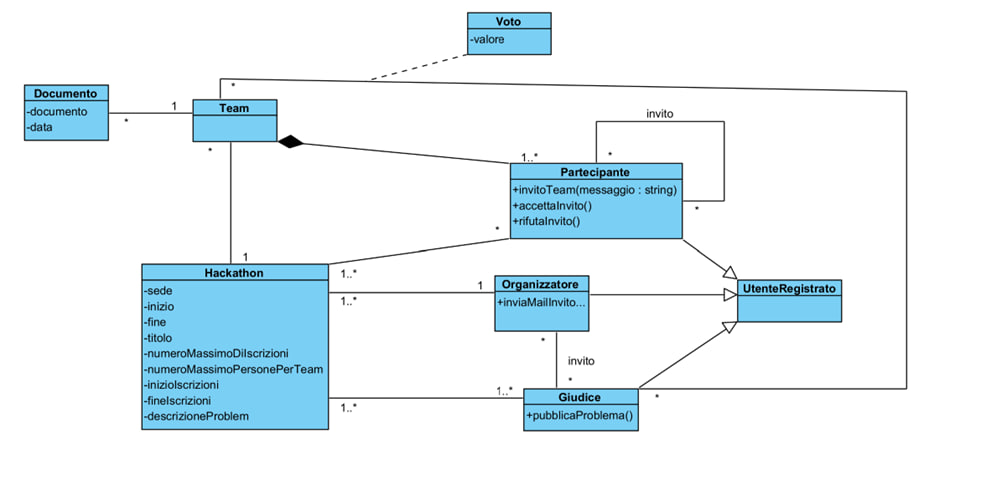
\includegraphics[width=1\textwidth]{Immagini/PossibileSoluzioneHackathon}
	\end{figure}
	
\end{document}
